\documentclass{beamer}
\usepackage[T1]{fontenc}
\usepackage[english]{babel}
\usefonttheme{serif}
\setbeamertemplate{navigation symbols}{
\usebeamerfont{footline}
\usebeamercolor[fg]{footline}
\insertframenumber/\inserttotalframenumber{}
}
\setbeamerfont{frametitle}{size = \small}
\usepackage{mathpazo}
\usepackage{float}
\usepackage[labelsep = colon]{caption}
\usepackage{amsmath}
\usepackage{setspace}
\usepackage{graphicx}
\usepackage{threeparttablex}
\usepackage{longtable}
\usepackage{booktabs}
\usepackage{dcolumn}
\usepackage{pdfpages}


\title{GV217 Conflict Analysis, Week 19}
\subtitle{Causes of Conflict: Feasibility \emph{versus} Grievance}
\author{Muzhou Zhang\\ muzhou.zhang@essex.ac.uk\\ Virtual Office Hour: 15:30--16:30, Friday, 997 5800 8679}
\date{11 Feb 2022}

\begin{document}
\maketitle
\setstretch{1.25}

\begin{frame}{Feasibility: External Oppertunities}
    \begin{itemize}
        \pause\item Economic --- oppertunity cost\\
        \pause      Initiating a civil war in Africa? ``\$10,000 and a satellite phone'' (Collier 2007)
        \pause\item Military
        \begin{itemize}
            \pause\item Geography
        \end{itemize}
    \end{itemize}
\end{frame}

\begin{frame}{Feasibility: External Oppertunities}
    \begin{center}
        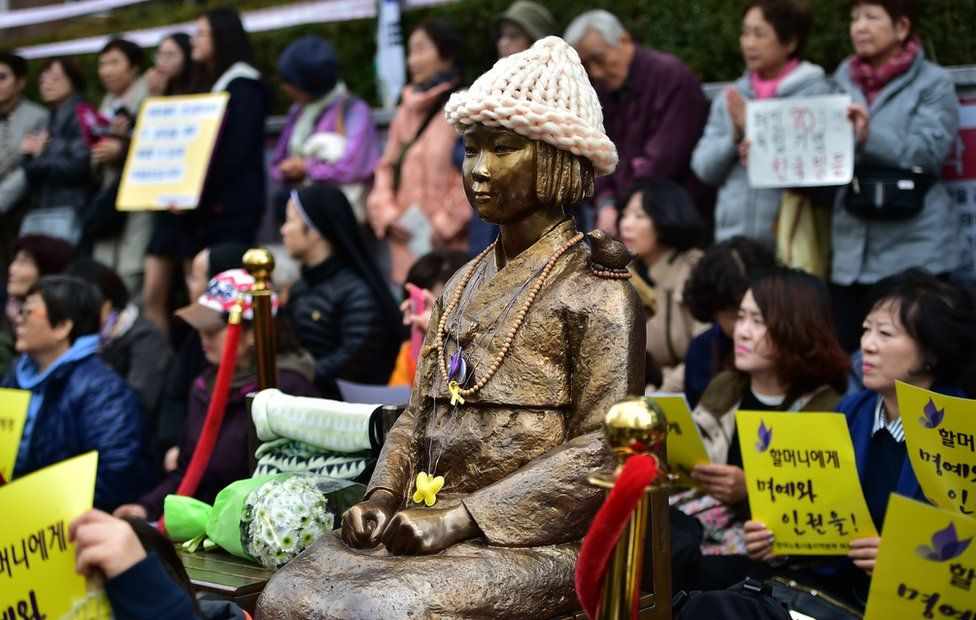
\includegraphics[width = \linewidth]{/Users/mz/Desktop/GitHub/teaching/gv217_conflict_analysis/figs/wk19/fig1.png}
    \end{center}
    \tiny Fabio Cuttica/Al Jazeera\\ \url{https://www.aljazeera.com/gallery/2015/12/12/farc-rebels-in-colombian-jungle}
\end{frame}

\begin{frame}{Feasibility: External Oppertunities}
    \begin{center}
        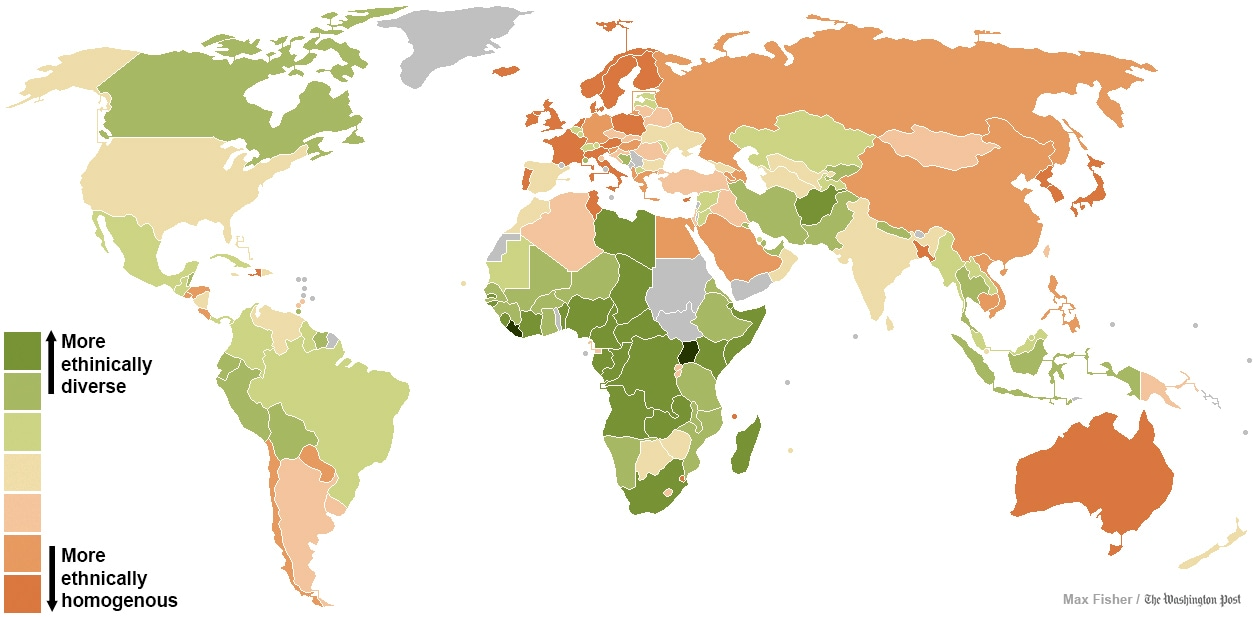
\includegraphics[width = \linewidth]{/Users/mz/Desktop/GitHub/teaching/gv217_conflict_analysis/figs/wk19/fig2.png}
    \end{center}
    \tiny Fabio Cuttica/Al Jazeera\\ \url{https://www.aljazeera.com/gallery/2015/12/12/farc-rebels-in-colombian-jungle}
\end{frame}

\begin{frame}{Feasibility: External Oppertunities}
    \begin{center}
        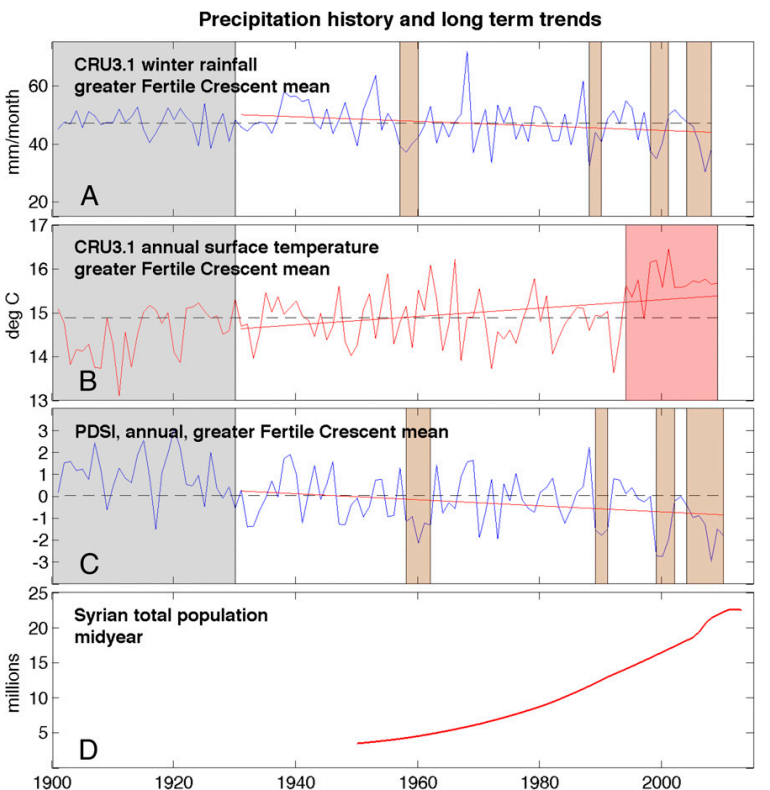
\includegraphics[width = \linewidth]{/Users/mz/Desktop/GitHub/teaching/gv217_conflict_analysis/figs/wk19/fig3.png}
    \end{center}
    \tiny Fabio Cuttica/Al Jazeera\\ \url{https://www.aljazeera.com/gallery/2015/12/12/farc-rebels-in-colombian-jungle}
\end{frame}

\begin{frame}{Feasibility: External Oppertunities}
    \begin{center}
        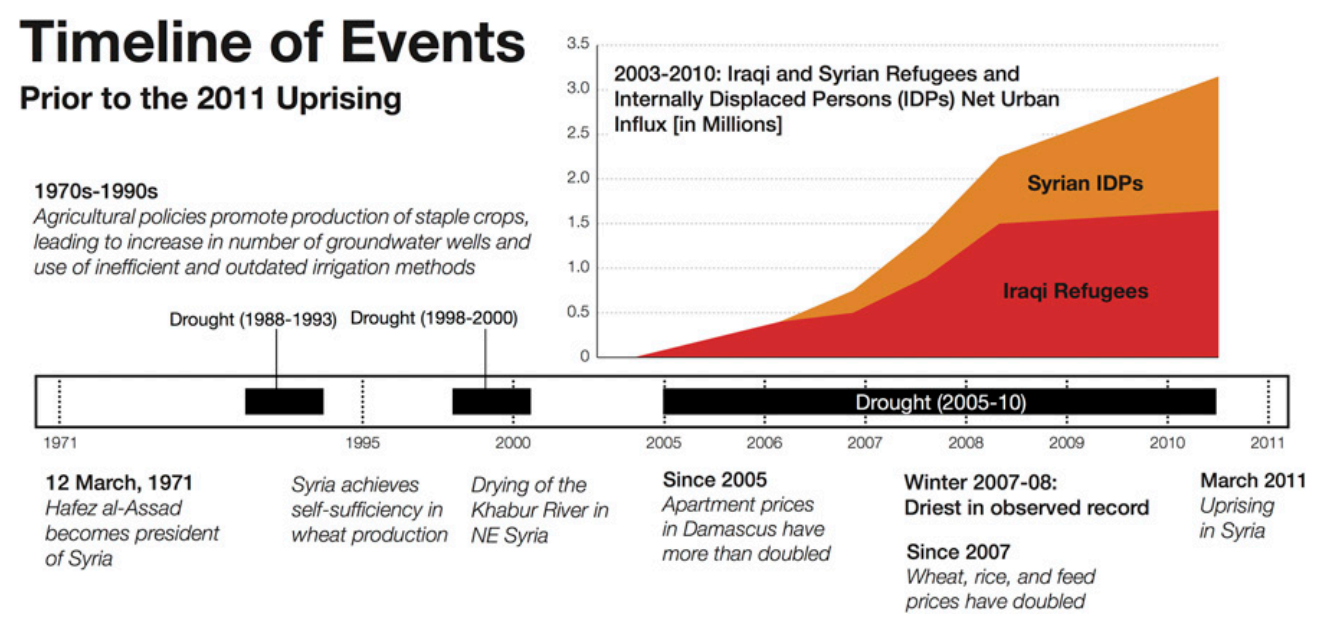
\includegraphics[width = \linewidth]{/Users/mz/Desktop/GitHub/teaching/gv217_conflict_analysis/figs/wk19/fig4.png}
    \end{center}
    \tiny Tyler Hicks/The New York Times\\ \url{https://www.nytimes.com/article/afghanistan-war-photos-pictures.html}
\end{frame}

\begin{frame}{Feasibility: External Oppertunities}
    \begin{center}
        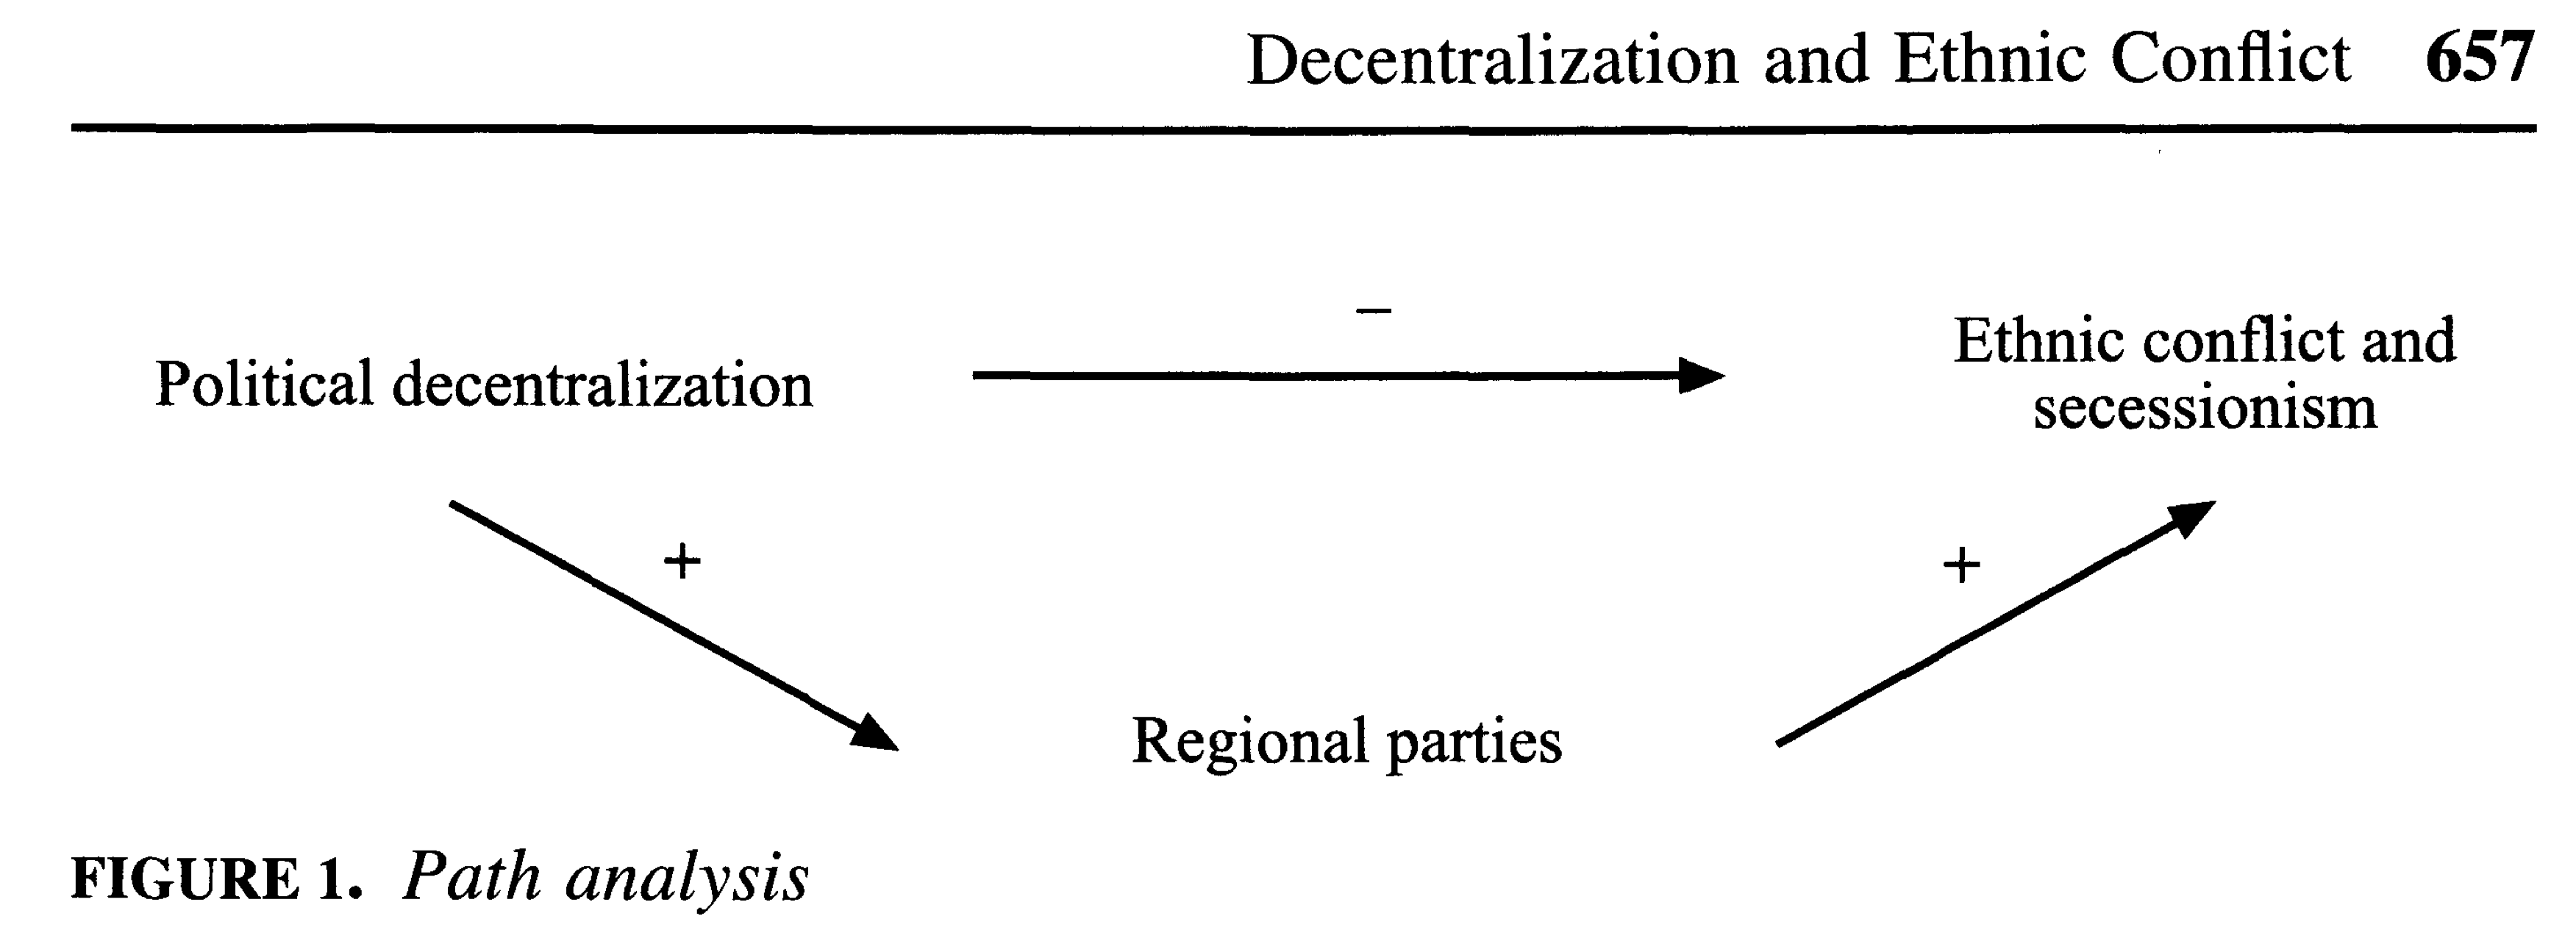
\includegraphics[width = \linewidth]{/Users/mz/Desktop/GitHub/teaching/gv217_conflict_analysis/figs/wk19/fig5.png}
    \end{center}
    \tiny Daniel Berehulak for The New York Times\\ \url{https://www.nytimes.com/article/afghanistan-war-photos-pictures.html}
\end{frame}

\begin{frame}{Feasibility: External Oppertunities}
    \begin{center}
        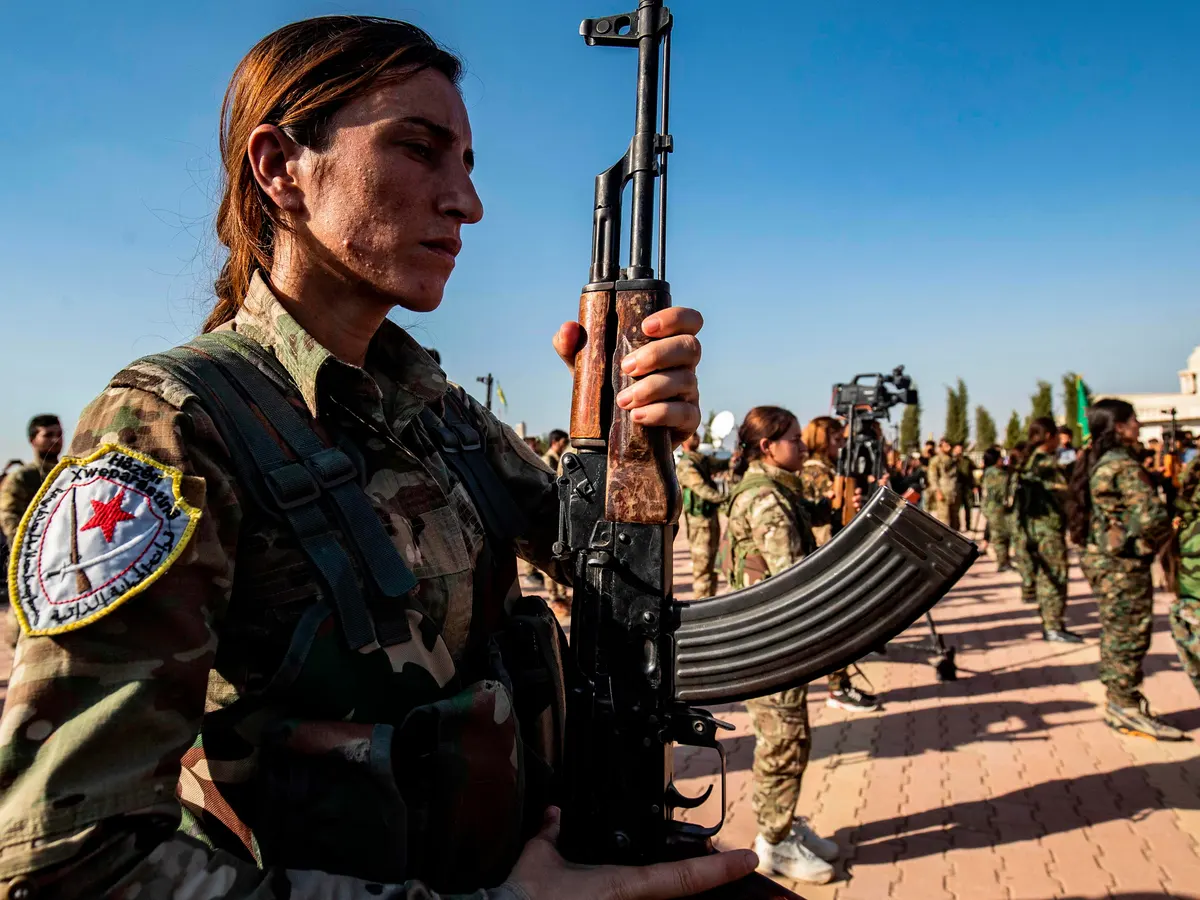
\includegraphics[width = \linewidth]{/Users/mz/Desktop/GitHub/teaching/gv217_conflict_analysis/figs/wk19/fig6.png}
    \end{center}
    \tiny Sergey Ponomarev for The New York Times\\ \url{https://www.nytimes.com/article/afghanistan-war-photos-pictures.html}
\end{frame}

\begin{frame}{Feasibility: External Oppertunities}
    \begin{itemize}
        \item Economic --- oppertunity cost\\
              Initiating a civil war in Africa? ``\$10,000 and a satellite phone'' (Collier 2007)
        \item Military
        \begin{itemize}
            \item Geography
            \item Previous conflicts --- path dependency
        \end{itemize}
    \end{itemize}
\end{frame}

\begin{frame}{Feasibility: External Oppertunities}
    \begin{center}
        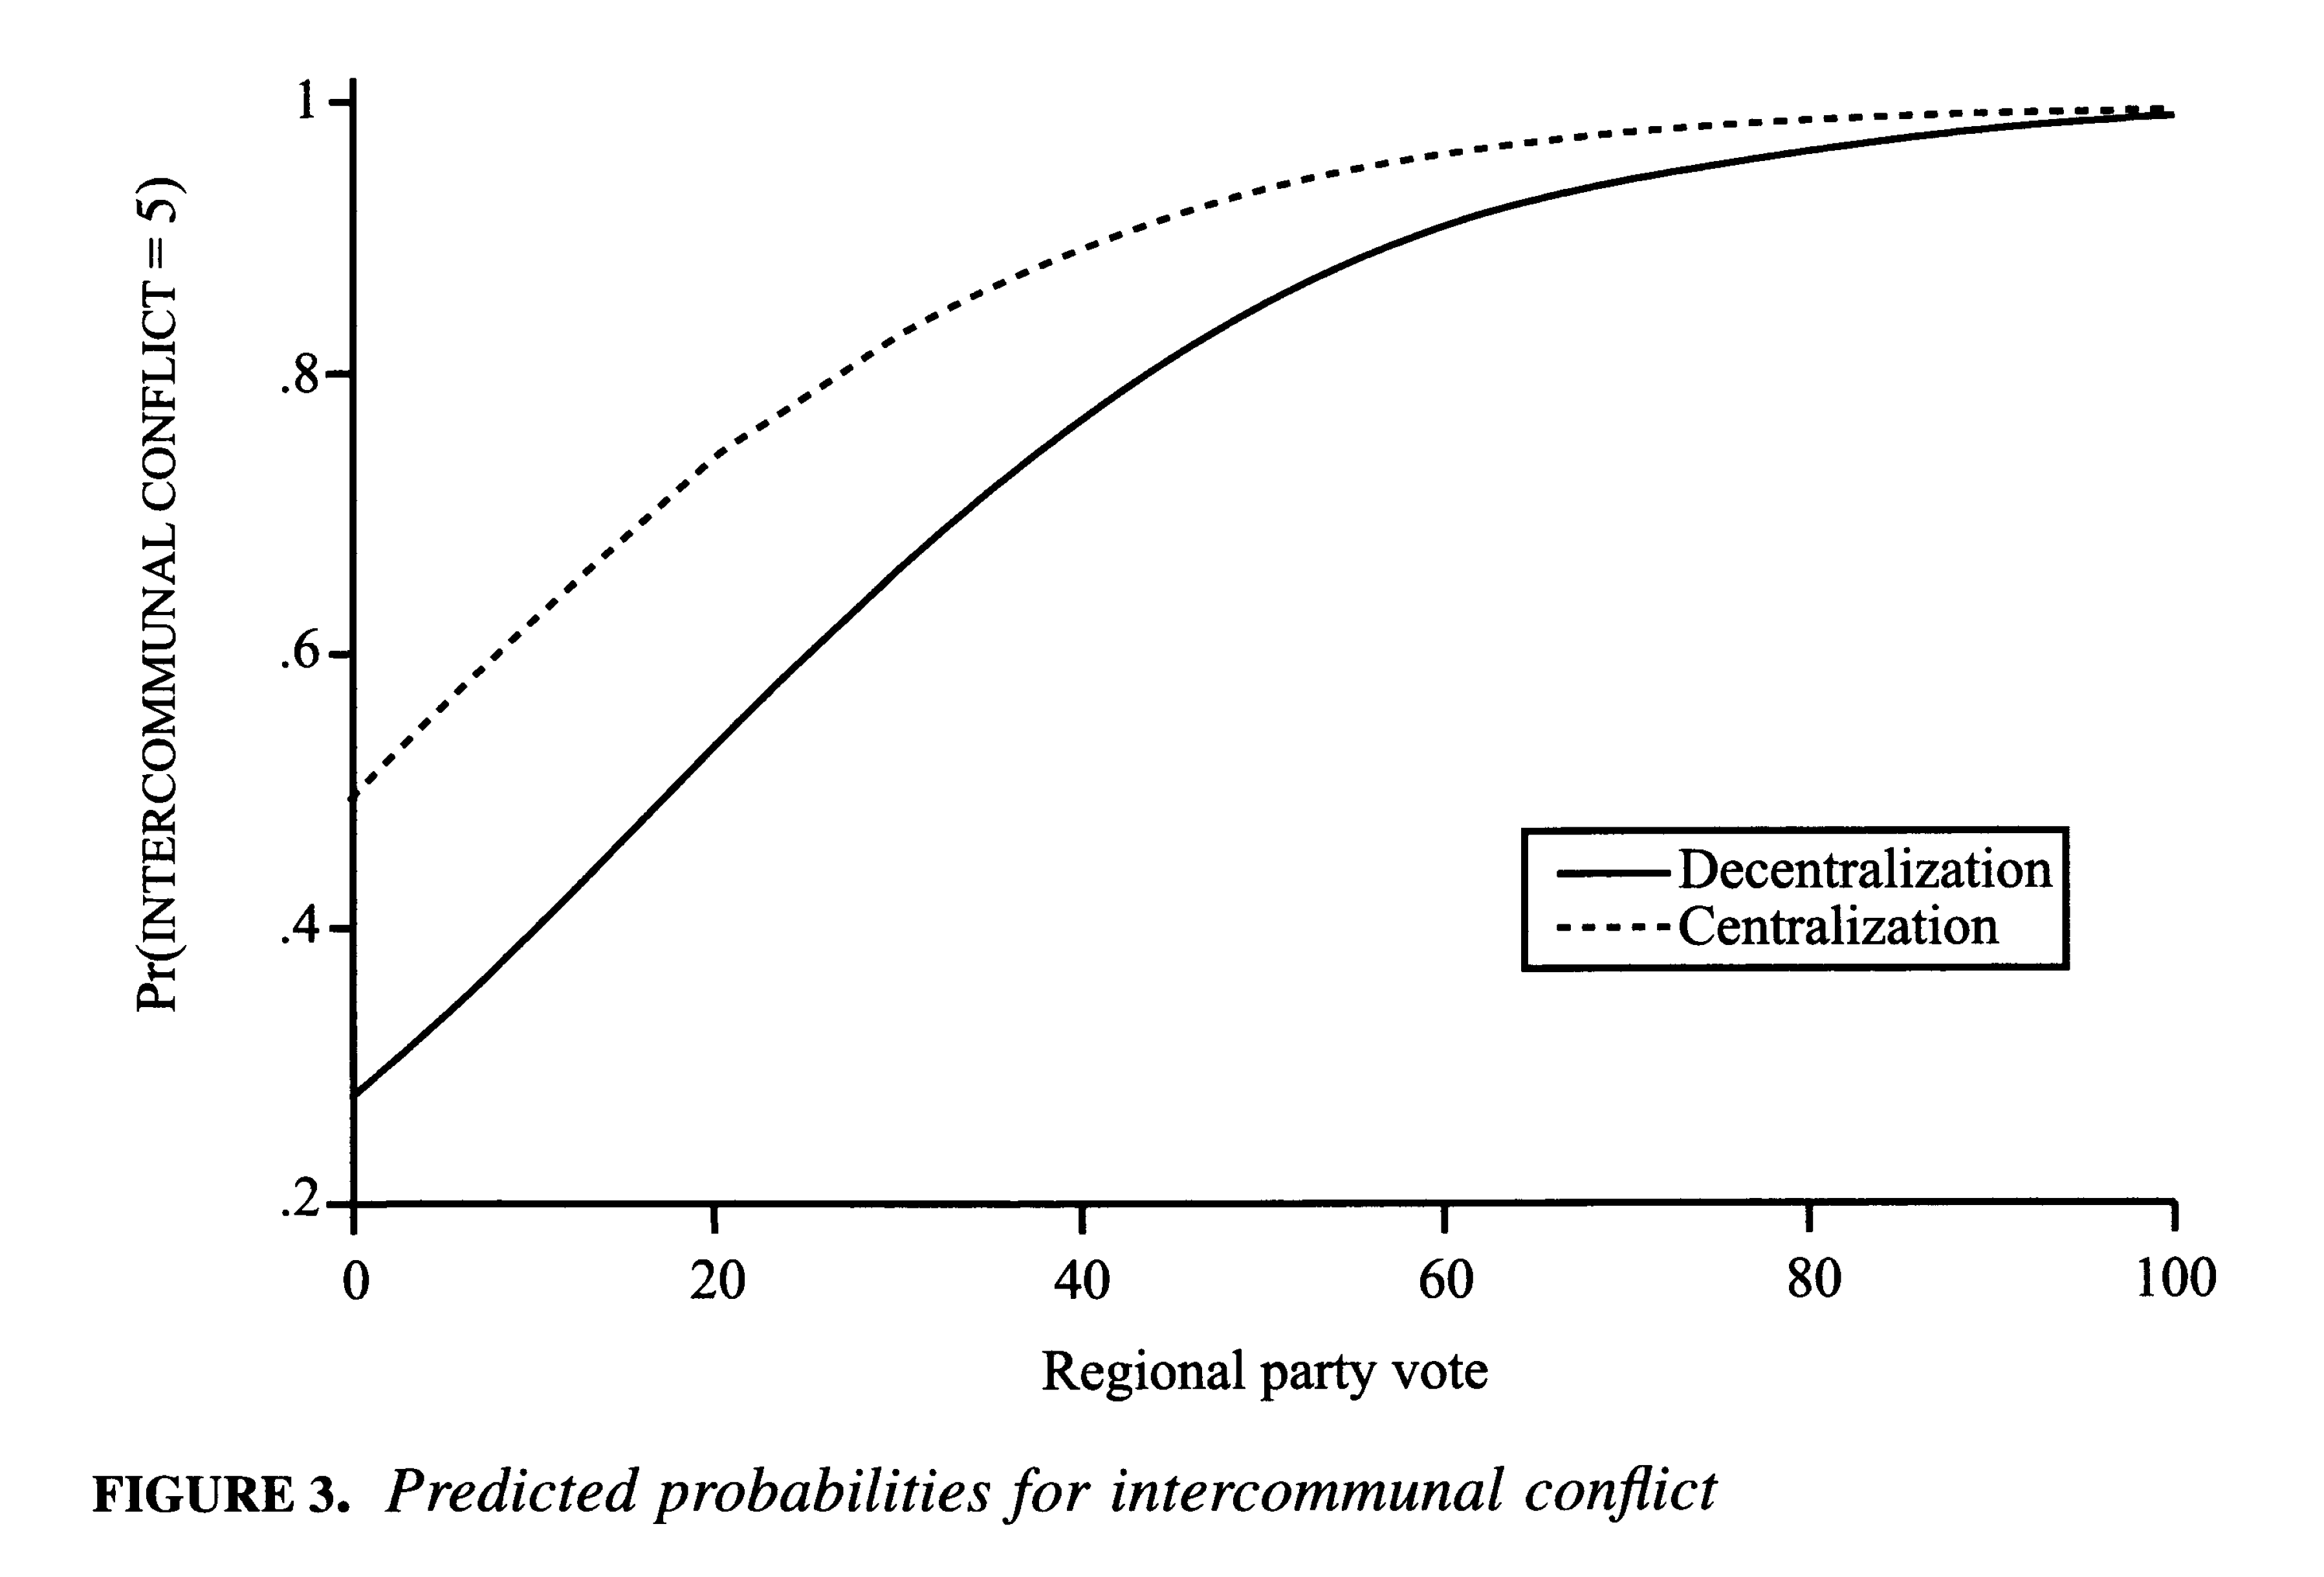
\includegraphics[width = \linewidth]{/Users/mz/Desktop/GitHub/teaching/gv217_conflict_analysis/figs/wk19/fig7.png}
    \end{center}
    \tiny Fernando Vergara/Associated Press\\ \url{https://www.nytimes.com/2017/08/03/opinion/farc-colombia.html}
\end{frame}

\begin{frame}{Grievance: Internal Motives}
    \begin{itemize}
        \pause\item Relative deprivation
        \pause\item Inequalitiy: vertical \emph{versus} horizontal
    \end{itemize}
\end{frame}

\begin{frame}{Grievance: Internal Motives}
    \pause
    \begin{center}
        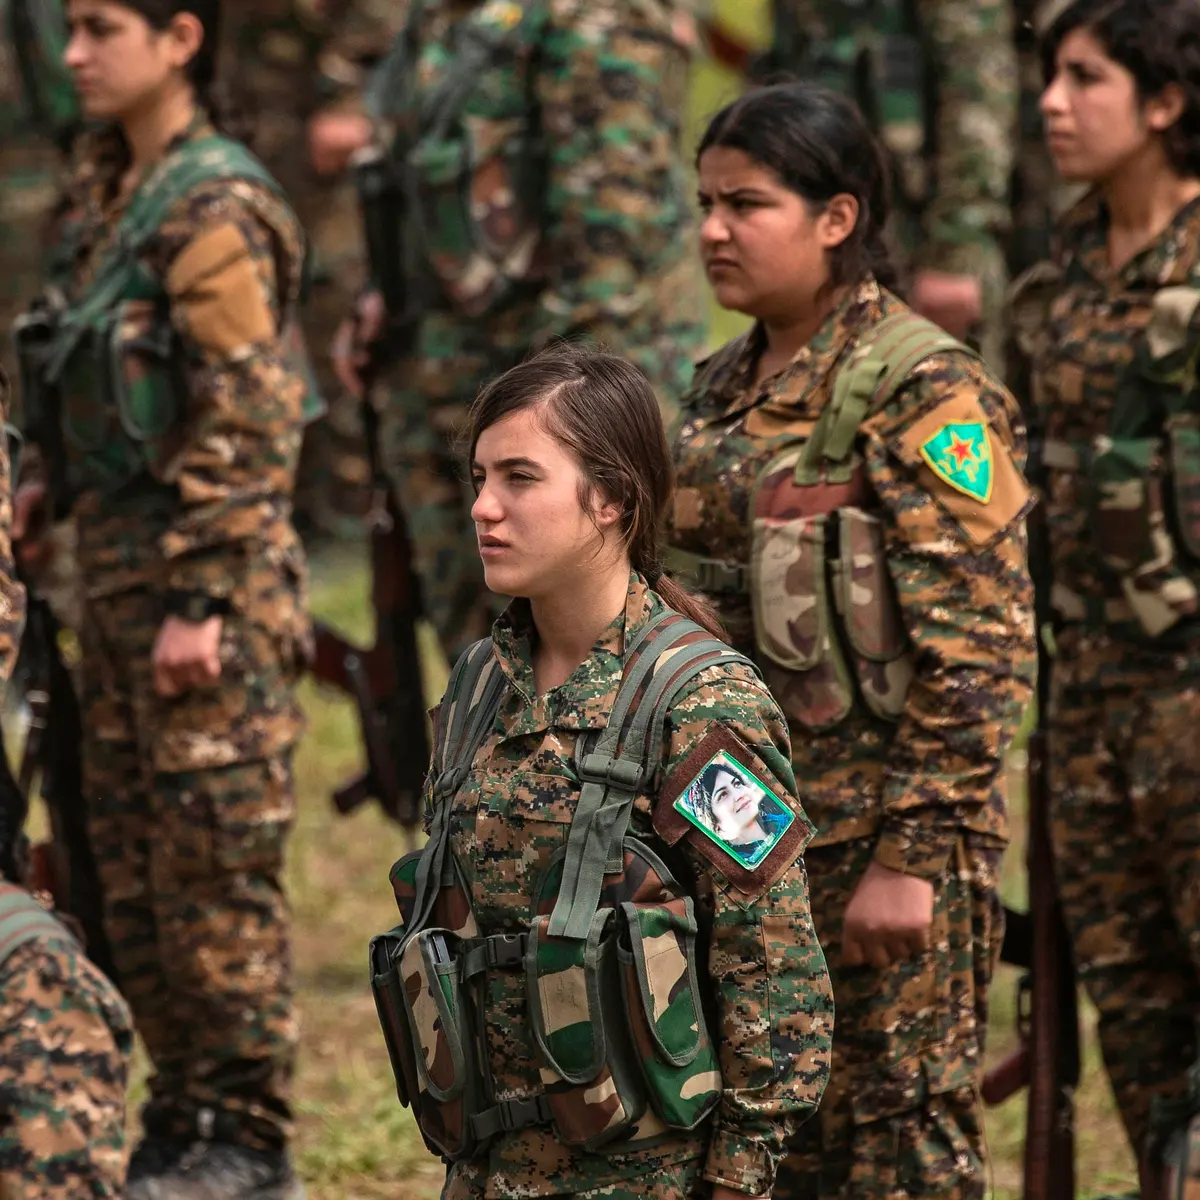
\includegraphics[width = \linewidth]{/Users/mz/Desktop/GitHub/teaching/gv217_conflict_analysis/figs/wk19/fig8.png}
    \end{center}
    \tiny The Economist\\ \url{https://tinyurl.com/5ef7w8x9}
\end{frame}

\begin{frame}{Collier, Hoeffler, \& Rohner (2009)}
    \pause
    \begin{center}
        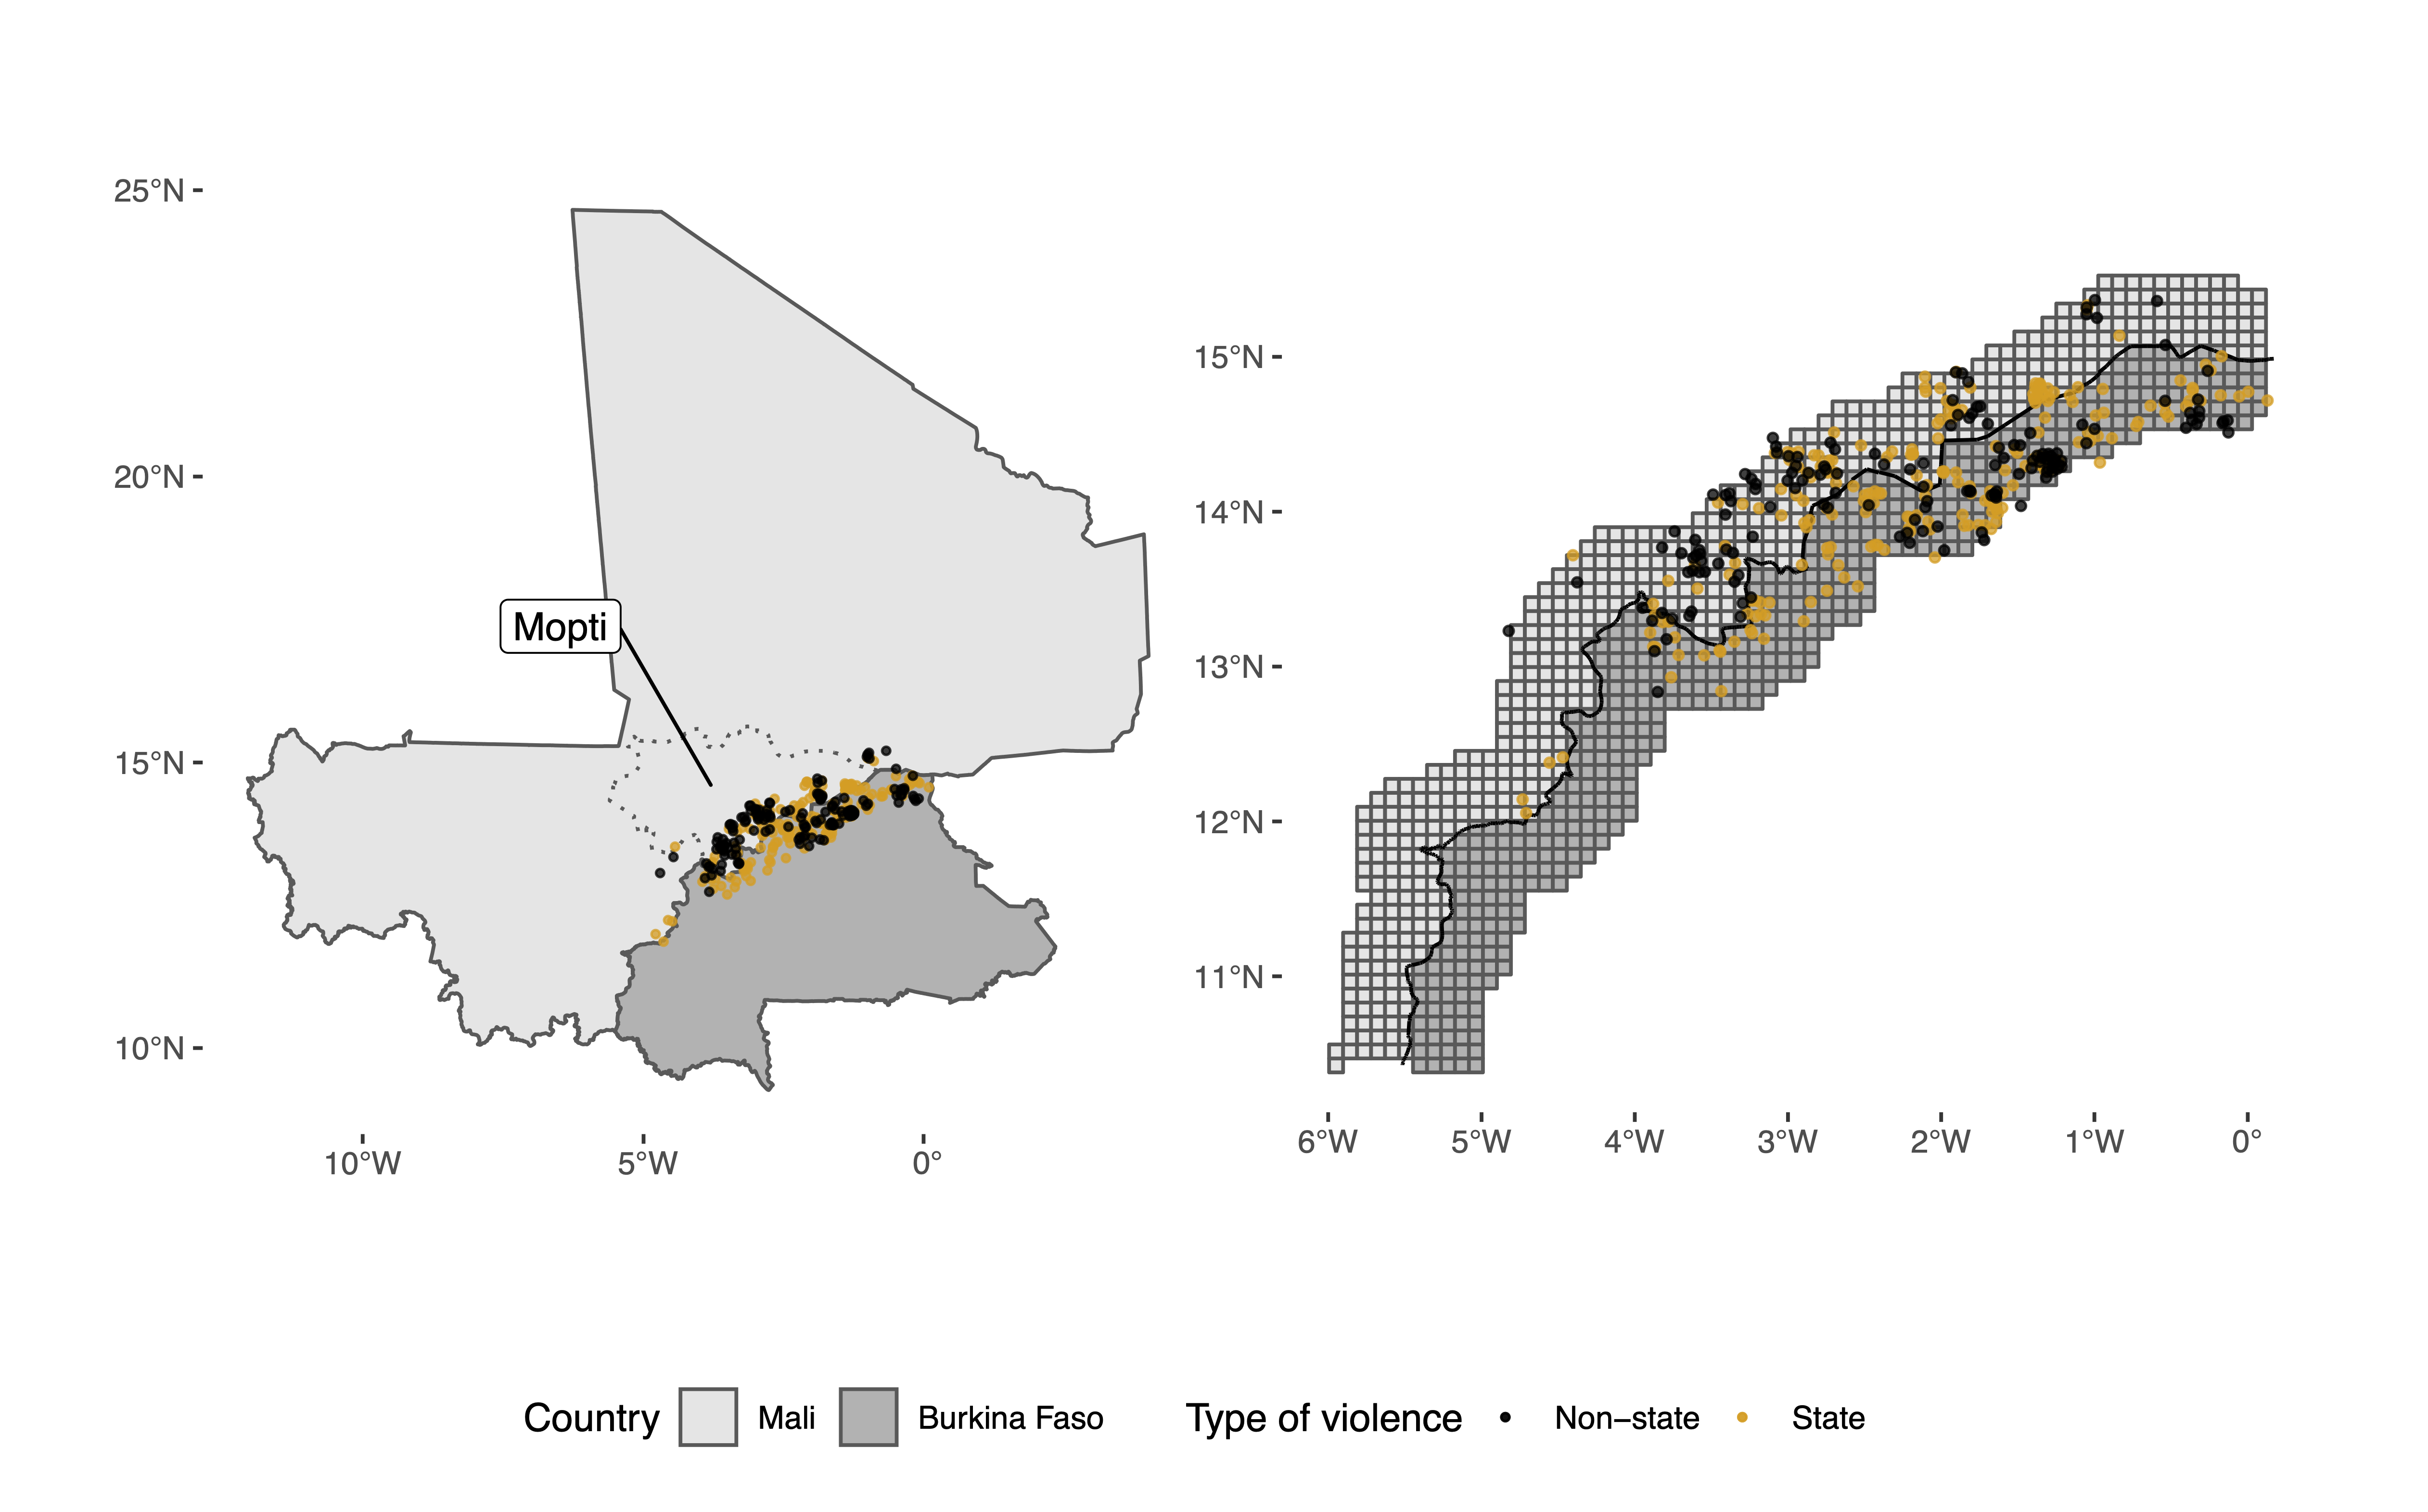
\includegraphics[width = \linewidth]{/Users/mz/Desktop/GitHub/teaching/gv217_conflict_analysis/figs/wk19/fig9.png}
    \end{center}
\end{frame}

\begin{frame}{Koubi \& Böhmelt (2014)}
    \pause
    \begin{center}
        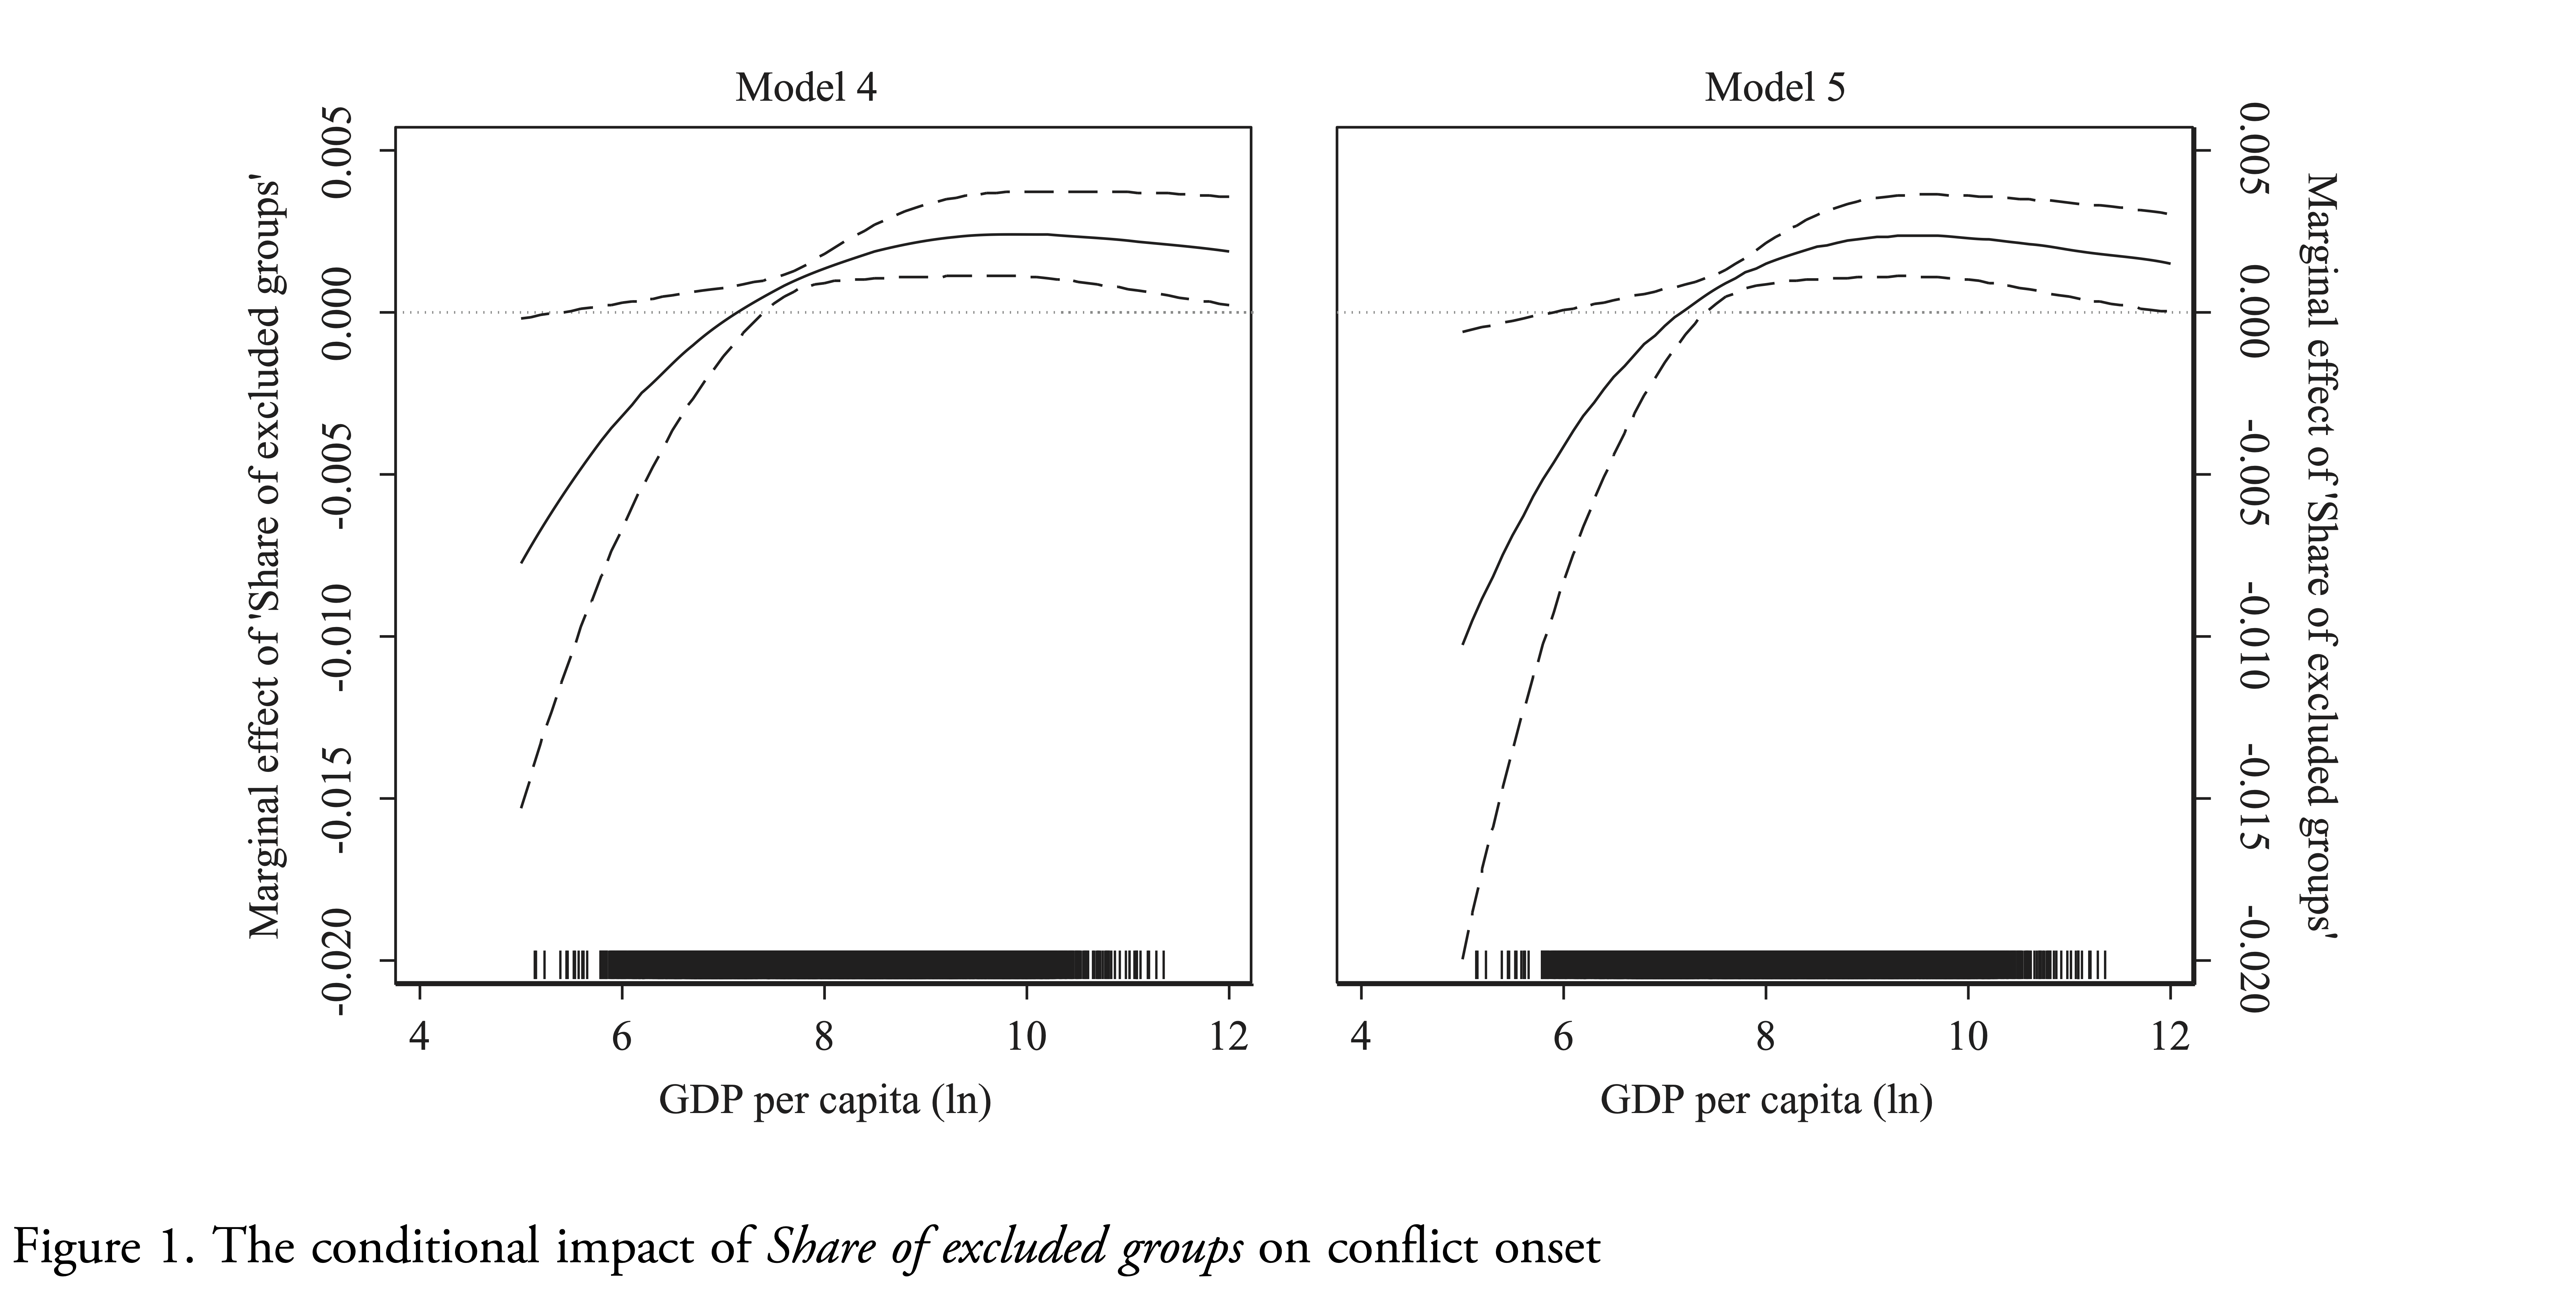
\includegraphics[width = \linewidth]{/Users/mz/Desktop/GitHub/teaching/gv217_conflict_analysis/figs/wk19/fig10.png}
    \end{center}
\end{frame}

\begin{frame}{Collier, Hoeffler, \& Rohner (2009); Koubi \& Böhmelt (2014)}
    \begin{itemize}
        \pause\item What are civil wars, and their data sources, in these two articles?
        \pause\item Are the units-of-analysis consistent with their theories?
        \pause\item Are the findings causal?
        \pause\item Is grievance and feasibility contradictory?
    \end{itemize}
\end{frame}

\begin{frame}{Resource Curse}
    \pause
    \begin{center}
        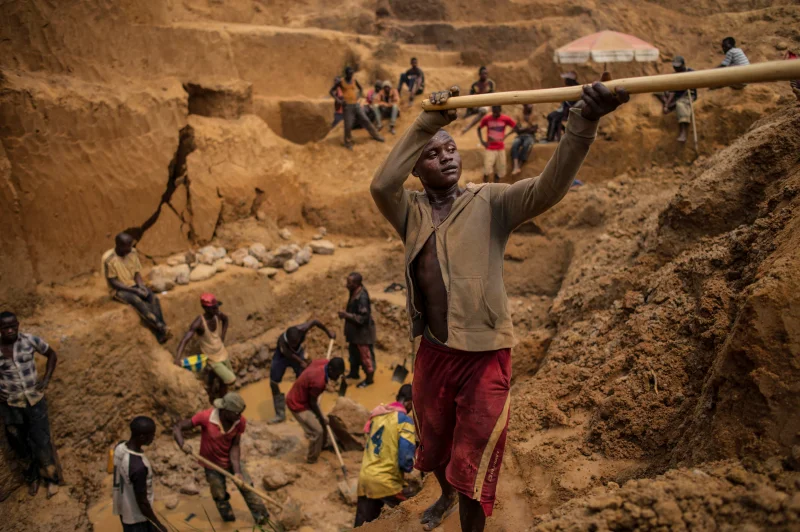
\includegraphics[width = \linewidth]{/Users/mz/Desktop/GitHub/teaching/gv217_conflict_analysis/figs/wk19/fig11.png}
    \end{center}
    \tiny Lynsey Addario (Getty Images) for TIME\\ \url{https://time.com/4012857/the-fight-against-blood-diamonds-continues/}
\end{frame}

\begin{frame}{Resource Curse}
    \pause
    \begin{center}
        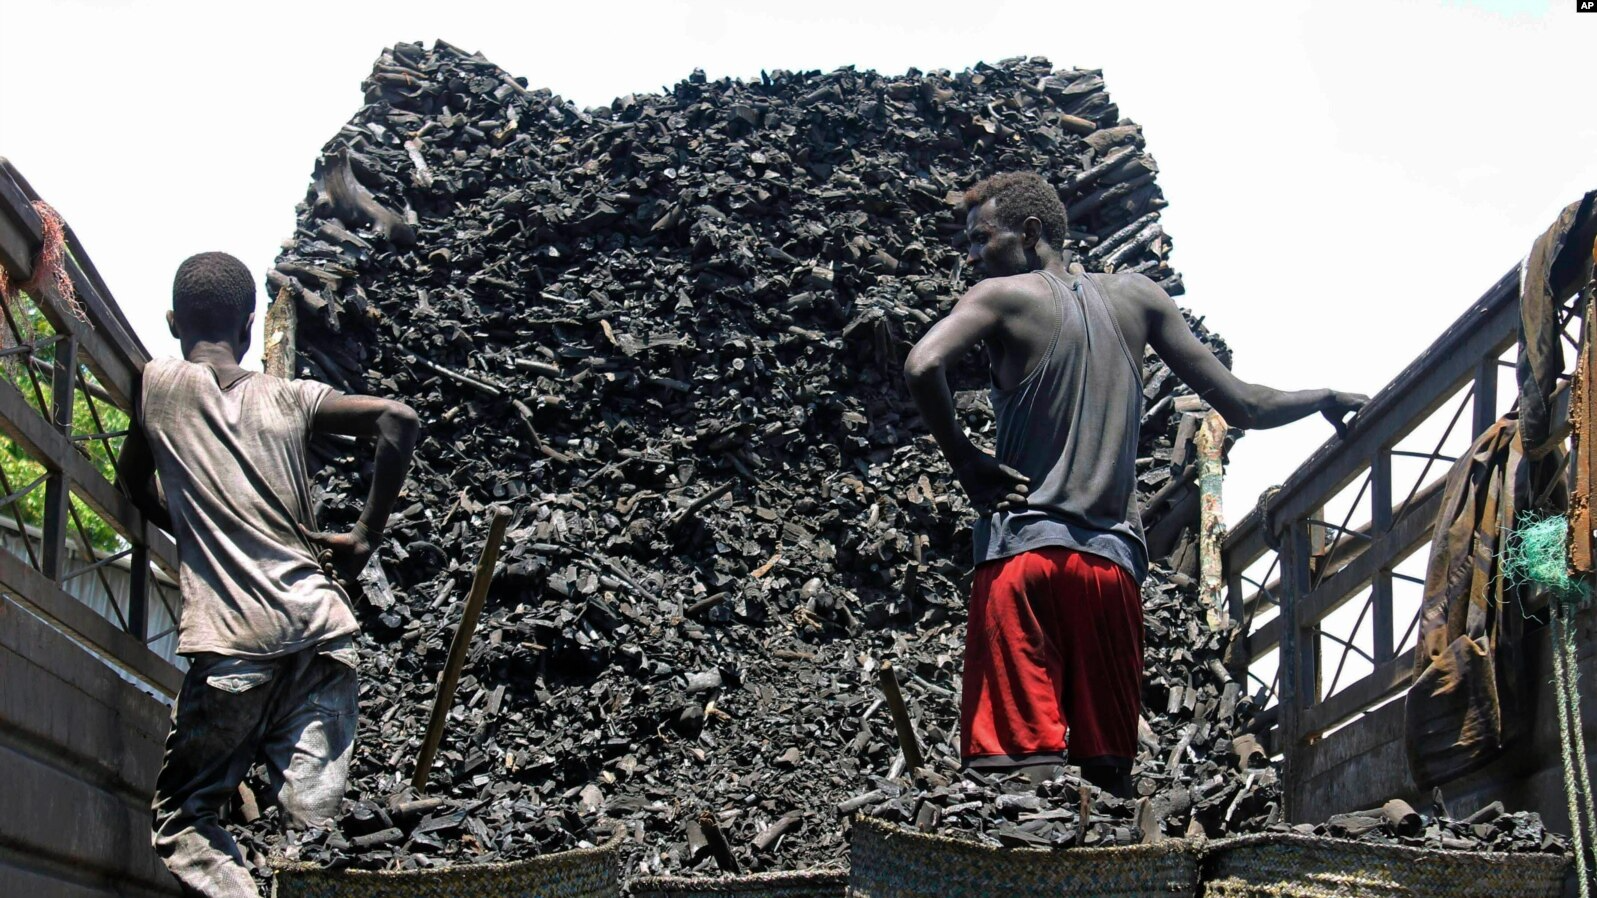
\includegraphics[width = \linewidth]{/Users/mz/Desktop/GitHub/teaching/gv217_conflict_analysis/figs/wk19/fig12.png}
    \end{center}
    \tiny Photo © AP\\ \url{https://tinyurl.com/2rtdbprx}
\end{frame}

\begin{frame}{Resource Curse}
    \begin{itemize}
        \pause\item Natural resources fund rebels (Collier, Hoeffler, \& Rohner 2009)
        \pause\item Do natural resources incentivize rebels? It's about the greed argument.
        \pause\item Do wind-fall revenues fuel grievance?
    \end{itemize}
\end{frame}

\end{document}
